\documentclass[UTF8,a4paper,11pt]{article}
\usepackage{times}
\usepackage{amsmath,amssymb}
\usepackage{bm}
\usepackage{ctex}
\usepackage{xcolor}


\usepackage{graphicx,epsfig,subfigure}
\usepackage{tikz}
\usetikzlibrary{backgrounds,automata}


\usepackage[utf8]{inputenc}


\begin{document}
\title{}
\author{}
\date{}
% \maketitle


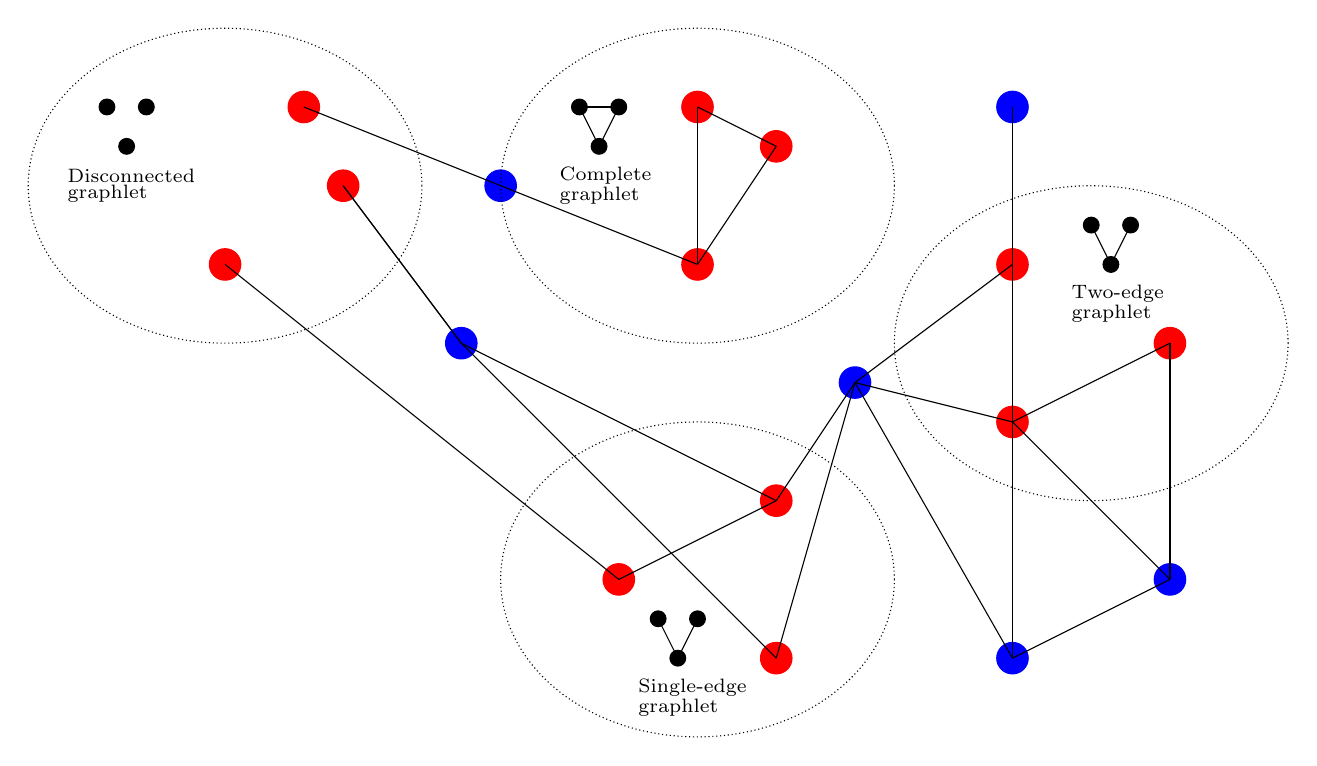
\begin{tikzpicture}

    % \draw [help lines, step = 1] (-10,-10) grid (10,10);
    % \filldraw (0,0) circle (0.1);

    \filldraw (-9,3) circle (0.1);
    \filldraw (-9.5,3) circle (0.1);
    \filldraw (-9.25,2.5) circle (0.1);
    \node [font = \fontsize{7}{4}\selectfont, text width=2cm] at (-9,2) {Disconnected graphlet};

    \filldraw (-3,3) circle (0.1);
    \filldraw (-3.5,3) circle (0.1);
    \filldraw (-3.25,2.5) circle (0.1);
    \draw (-3,3)--(-3.5,3);
    \draw (-3,3)--(-3.25,2.5);
    \draw (-3.5,3)--(-3.25,2.5);
    \node [font = \fontsize{7}{4}\selectfont, text width=2cm] at (-2.75,2) {Complete graphlet};

    \filldraw (3,1.5) circle (0.1);
    \filldraw (3.5,1.5) circle (0.1);
    \filldraw (3.25,1) circle (0.1);
    \draw (3,1.5)--(3.25,1);
    \draw (3.5,1.5)--(3.25,1);
    \node [font = \fontsize{7}{4}\selectfont, text width=2cm] at (3.75,0.5) {Two-edge graphlet};

    \filldraw (-2,-3.5) circle (0.1);
    \filldraw (-2.5,-3.5) circle (0.1);
    \filldraw (-2.25,-4) circle (0.1);
    \draw (-2,-3.5)--(-2.25,-4);
    \draw (-2.5,-3.5)--(-2.25,-4);
    \node [font = \fontsize{7}{4}\selectfont, text width=2cm] at (-1.75,-4.5) {Single-edge graphlet};

    % circle1
    \filldraw [red] (-7,3) circle (0.2);
    \filldraw [red] (-6.5,2) circle (0.2);
    \filldraw [red] (-8,1) circle (0.2);

    % circle2
    \filldraw [red] (-2,3) circle (0.2);
    \filldraw [red] (-1,2.5) circle (0.2);
    \filldraw [red] (-2,1) circle (0.2);
    \filldraw [blue] (-4.5,2) circle (0.2);

    % circle3
    \filldraw [red] (2,1) circle (0.2);
    \filldraw [red] (2,-1) circle (0.2);
    \filldraw [red] (4,0) circle (0.2);

    % circle4
    \filldraw [red] (-3,-3) circle (0.2);
    \filldraw [red] (-1,-2) circle (0.2);
    \filldraw [red] (-1,-4) circle (0.2);

    % out blue
    \filldraw [blue] (0,-0.5) circle (0.2);
    \filldraw [blue] (2,3) circle (0.2);
    \filldraw [blue] (-5,0) circle (0.2);
    \filldraw [blue] (2,-4) circle (0.2);
    \filldraw [blue] (4,-3) circle (0.2);

    % circle
    \draw [densely dotted] (-8,2) ellipse (2.5 and 2);
    \draw [densely dotted] (-2,2) ellipse (2.5 and 2);
    \draw [densely dotted] (3,0) ellipse (2.5 and 2);
    \draw [densely dotted] (-2,-3) ellipse (2.5 and 2);

    \draw (-2,3)--(-1,2.5);
    \draw (-2,3)--(-2,1);
    \draw (-1,2.5)--(-2,1);

    \draw (-7,3)--(-4.5,2);
    \draw (-4.5,2)--(-2,1);
    \draw (-6.5,2)--(-5,0);

    \draw (-8,1)--(-3,-3);
    \draw (-5,0)--(-1,-2);
    \draw (-1,-2)--(0,-0.5);

    \draw (-1,-4)--(-5,0);
    \draw (-1,-4)--(0,-0.5);
    \draw (-6.5,2)--(-5,0);

    \draw (-3,-3)--(-1,-2);
    \draw (0,-0.5)--(2,-4);
    \draw (0,-0.5)--(2,1);

    \draw (0,-0.5)--(2,-1);
    \draw (2,-1)--(2,1);
    \draw (2,-1)--(4,0);

    \draw (2,-4)--(4,-3);
    \draw (4,-3)--(4,0);
    \draw (4,-3)--(2,-1);

    \draw (2,-4)--(2,-1);
    \draw (2,1)--(2,3);

    


\end{tikzpicture}




\end{document}



% \begin{document}

% \begin{tikzpicture}
%     \draw (1,1) ellipse (2 and 3)
%     \draw [densely dotted]

% \end{tikzpicture}

% \end{document}


